\section{~Wave Model Structure and Data Flow} \label{chapt:run}
\newcounters

\vsssub
\subsection{~Program design} \label{run:design}
\vssub

The core of \ws\ is the wave model subroutine, which can be
called by either a stand-alone program shell or any other program that
requires dynamically updated wave data. Two such programs are provided with
the \ws\ release (e.g., {\code ww3\_shel} and {\code ww3\_multi}). 
Auxiliary programs include a grid preprocessor {\code ww3\_grid}, a program to
generate artificial initial conditions {\code ww3\_strt}, generic program shells
for individual {\code ww3\_shel} or multi-grid {\code ww3\_multi} applications,
two input pre-processors ({\code ww3\_prep} and {\code ww3\_prnc}), and  
post-processors for gridded ({\code ww3\_outf} and {\code ww3\_ounf}) and point 
({\code ww3\_outp} and {\code ww3\_ounp}) output data.

In this section, note that file names will be identified by the {\file
file} type font, the contents of a file by the {\code code} type font and {\sc
fortran} program elements by the {\F fortran} type font. The main wave model 
subroutine is {\F w3wave}. Data files are identified with the
file extension {\file .ww3}, except in the multi-grid wave model {\file
ww3\_multi}, where the file extension identifies individual grids part of a chosen
multi-grid mosaic. For simplicity, the file extension {\file .ww3} will be used 
throughout this chapter.  

A relational diagram including the basic data flow is presented in 
Fig.~\ref{fig:run_elements}. The figure illustrates a typical workflow, as follows.
 The grid pre-processor {\code ww3\_grid} writes a model definition file {\file mod\_def.ww3} with
bottom and obstruction information and parameter values defining the physical
and numerical approaches. The wave model may have cold or hot starts. 
Hot starting requires a restart file {\file restart.ww3}, created either
by the wave model itself in a previous run, or by the initial conditions program {\code ww3\_strt}.
If a restart file is not available, the wave model will be initialized automatically.
If linear growth or spectral seeding is switch on, the model may start from a flat ocean ($H_s
= 0$), otherwise the initial conditions will consist of a parametric
fetch-limited spectrum based on the initial wind field (see the corresponding
option in the initial conditions program).  

The wave model routine ({\F
  w3wave}) optionally generates up to 9 restart files {\file
  restart{\em{n}}.ww3}, where {\file{\em{n}}} represents a single digit
integer number. For telescoping nest applications, the wave model also 
optionally reads boundary conditions from
the file {\file nest.ww3} and generates boundary conditions for consecutive
nested runs in {\file nest{\em{n}}.ww3}. The model furthermore dumps raw data to the
output files {\file out\_grd.ww3 }, {\file out\_pnt.ww3}, {\file track\_o.ww3}
and {\file partition.ww3} (gridded mean wave parameters, spectra at locations,
spectra along tracks, and partitioned wave data, respectively). The tracks
along which spectra are to be presented is defined in the file {\file
  track\_i.ww3}. Note that the wave model does not write to standard output,
because this would be inconvenient if \ws\ is part of an integrated
model. Instead, it maintains its own log file {\file log.ww3} and optionally a
test output files {\file test.ww3} for a shared memory version of the model,
or {\file test{\em{nnn}}.ww3} for distributed memory versions, where {\em nnn}
is the processor number starting with 1.  Finally, various output
post-processors are available (binary post-processing of raw gridded fields,
point output and track output files; NetCDF and GRIB(2) packing of wave data;
post-processing for later GrADS graphical processing of gridded and spectral
data). A more detailed description of all program elements and their input
files is given below. Note that the source codes of each routine are fully
documented. This documentation is an additional source of information about
\ws.

\setlength{\unitlength}{0.1mm}
\begin{figure}

\begin{picture}(1370,1080)(0,-1080)

\put(  50,  -80){\dashbox{5}(280,80)[c]{{\file grid data}}}
\put( 190,  -80){\vector(0,-1){60}}

\put(   0, -220){\framebox(380,80)[c]{grid preprocessor}}
\put( 190, -220){\vector(0,-1){60}}

\put(  50, -360){\dashbox{5}(280,80)[c]{{\file mod\_def.ww3}}}
\put( 190, -360){\vector(0,-1){380}}
\put( 190, -460){\vector(1,0){60}}
\put( 330, -320){\line(1,0){560}}
\put( 890, -320){\vector(1,1){100}}
\put( 890, -320){\line(1,-1){80}}
\put( 970, -400){\vector(0,-1){160}}

\put( 250, -500){\framebox(280,80)[c]{initial cond.}}
\put( 530, -460){\vector(1,0){60}}

\put( 590, -500){\dashbox{5}(280,80)[c]{{\file restart.ww3}}}
\put( 870, -500){\vector(1,-1){60}}

\put( 590, -640){\makebox(280,80)[c]{{\file restart.ww3}}}
\put( 590, -680){\makebox(280,80)[c]{{\file nest.ww3}}}
\put( 590, -680){\dashbox{5}(280,120)[c]{ }}

\put( 930, -640){\dashbox{10}(280,80)[c]{{\code wave model}}}
\put( 930, -600){\vector(-1,0){60}}
\put( 870, -600){\vector(1,0){60}}

\put( 590, -860){\makebox(280,80)[c]{{\file partition.ww3}}}
\put( 590, -780){\makebox(280,80)[c]{{\file out\_pnt.ww3}}}
\put( 590, -820){\makebox(280,80)[c]{{\file out\_grd.ww3}}}
\put( 590, -860){\dashbox{5}(280,170)[c]{ }}
\put( 970, -780){\vector(-1,0){100}}
\put( 590, -780){\vector(-1,0){60}}

\put( 970, -640){\vector(0,-1){240}}
\put( 830, -960){\makebox(280,80)[c]{{\file log.ww3}}}
\put( 830,-1000){\makebox(280,80)[c]{{\file test.ww3}}}
\put( 830,-1000){\dashbox{5}(280,120)[c]{ }}

\put(1170, -640){\vector(0,-1){100}}
\put(1170, -740){\vector(0,1){100}}
\put(1030, -820){\makebox(280,80)[c]{{\file track\_i.ww3}}}
\put(1030, -860){\makebox(280,80)[c]{{\file track\_o.ww3}}}
\put(1030, -860){\dashbox{5}(280,120)[c]{ }}

\put( 150, -820){\makebox(380,80)[c]{output}}
\put( 150, -860){\makebox(380,80)[c]{postprocessing}}
\put( 150, -860){\framebox(380,120)[c]{ }}

\put(1020, -560){\line(0,1){280}}
\put(1020, -280){\line(1,0){320}}
\put(1210, -620){\line(1,0){130}}
\put(1340, -620){\line(0,1){340}}
\put(1020, -370){\makebox(320,80)[c]{program}}
\put(1020, -410){\makebox(320,80)[c]{shell}}
\put(1020, -450){\makebox(320,80)[c]{or}}
\put(1020, -490){\makebox(320,80)[c]{integrated}}
\put(1020, -540){\makebox(320,80)[c]{program}}

\put(1040,  -80){\dashbox{5}(280,80)[0,0]{{\file input files}}}
\put(1170,  -80){\vector(0,-1){60}}

\put( 990, -220){\framebox(380,80)[c]{input preprocessor}}
\put(1170, -220){\vector(0,-1){60}}

{\scriptsize
\put(  50,-1010){\dashbox{5}(150,40)[0,0]{{\file file}}}
\put( 240,-1010){\dashbox{10}(150,40)[c]{{\code subrout.}}}
\put( 430,-1010){\framebox(150,40)[c]{program}}
\put( 140,-1050){\vector(1,0){60}}
\put( 220,-1070){\makebox(400,40)[l]{data transfer by file}}
\put(   0,-1090){\framebox(630,150){ }}                 }

\end{picture}

\caption{Basic program elements and data flow.}
\label{fig:run_elements}

\botline

\end{figure}


Files specific to \ws\ are opened by name within program subroutines. The unit
numbers, however, are defined by the user\footnote{~Except for {\file
ww3\_multi}.} within each {\file \.inp}, guaranteeing the largest possible 
flexibility for implementation in integrated models.

In addition to the wave model subroutine, an initialization routine and an interface
routine for data assimilation are provided. The routine includes a
generic interface that provides all necessary model components to perform full
spectral data assimilation. This routine is integrated into the generic wave
model shell, which is set up to perform time step managements for a wave model
with or without data assimilation. The shell also provides a simple yet
flexible way to provide the data assimilation scheme with various types of
data. Data assimilation has not yet been included in the multi-grid wave model
shell.

\vssub
\subsection{~The wave model routines} \label{sec:core}
\vssub

The wave model driver is a subroutine within the \ws\ framework package. 
To run the model driver subroutine, a program shell is needed. 
\ws\ is provided with a simple stand-alone shell as
will be discussed in \para\ref{sec:ww3shel}, and with a more complex
multi-grid model shell as will be discussed in \para\ref{sec:ww3multi}. The
present section concentrates on the wave model driver subroutines.

The wave model initialization routine {\F w3init} performs model
initialization for a single wave model grid. This includes setting up part of
the I/O system by defining unit numbers, initializing internal time
management, processing the model definition file ({\file mod\_def.ww3}),
processing initial conditions ({\file restart.ww3}), preparing model output,
and calculating grid-dependent parameters. If the model is compiled for an
\mpi\ environment, all necessary communication for both calculations and
output are determined and initialized (the model uses persistent \mpi\
communication throughout).

The wave model routine {\F w3wave} can be called any number of times to
propagate the wave field for a single grid in time after the initialization
has taken place. After some initial checks, the subroutine interpolates winds
and currents, updates ice concentrations and water levels, propagates the wave
field, and applies the selected source terms for a number of time steps. The
internal time step is defined by the interval for which the calculations are
to be performed, and by the requested output times. At the end of the
calculations, the routine provides the calling program with the requested
fields of wave data. A documentation of the interface of {\F w3wave} can be
found in the source code ({\file w3wavemd.ftn}).

\begin{figure}
{\small \begin{verbatim}
                                    |    input    |     output    |
                                    |-------------|---------------|
  step | pass |    date      time   | b w l c i d | g p t r b f c |
-------|------|---------------------|-------------|---------------|
    0  |   1  | 1968/06/06 00:00:00 |   F         | X X           |
    8  |   1  |            02:00:00 |             |   X           |
   12  |   1  |            03:00:00 |             | X             |
   16  |   1  |            04:00:00 |             |   X           |
   24  |   1  |            06:00:00 |   X         | X X           |
   32  |   2  |            08:00:00 |             |   X           |
   36  |   2  |            09:00:00 |             | L             |
   40  |   2  |            10:00:00 |             |   X           |
   48  |   2  |            12:00:00 |   X       X |   L   L       |
-------+------+---------------------+-------------+---------------+ 
\end{verbatim} }
\caption{Example action table from file {\file log.ww3}.} \label{fig:log}
\botline
\end{figure}
 

Apart from the raw data files as described above, the program maintains a log
file {\file log.ww3}. This file is opened by {\F w3init} (contained in {\F
  w3wave} in {\file w3wavemd.ftn}), which writes some self-explanatory header
information to this file. Each consecutive call to {\F w3wave} adds several
lines to an `action table' in this log file as is shown in
Fig.~\ref{fig:log}. The column identified as `step' shows the discrete time
step considered. The column identified as `pass' identifies the sequence
number of the call to {\F w3wave}; i.e., 3 identifies that this action took
place in the third call to {\F w3wave}. The third column shows the ending time
of the time step. In the input and output columns the corresponding actions of
the model are shown. A {\tt X} identifies that the input has been updated, or
that the output has been performed. A {\tt F} indicates a first field read,
and an {\tt L} identifies the last output. The seven input columns identify
boundary conditions ({\tt b}), wind fields ({\tt w}), water levels ({\tt l}),
current fields ({\tt c}), ice concentrations ({\tt i}), and data for
assimilation ({\tt d}), respectively. Note that data assimilation takes place
at the end of the time step after the wave routine call. The seven output
columns identify gridded output ({\tt g}), point output ({\tt p}), output
along tracks ({\tt t}), restart files ({\tt r}), boundary data ({\tt b}), and
partitioned spectral data ({\tt f}), and output for coupling ({\tt c}),
respectively.

For the multi-grid wave model \citep[][{\file ww3\_multi}]{tol:OMOD08b} a set
of routines is build around the basic wave model routines. The three main
routines are the initialization routine {\F wminit}, a time stepping routine
{\F wmwave} and a finalization routine {\F wmfinl}, with similar functions as
the routines for a single grid as described above. Note that the raw input and
output files are generated for separate grid in the mosaic, and are identified
by replacing the standard file extension '{\file .ww3}' with a unique
identifier for each individual grid as chosen by the user in the 
{\file ww3\_grid.inp} file. Log files are maintained for each individual grid, 
as well as an overall log file {\file log.mww3}.

\vssub
\subsection{~The data assimilation interface} \label{sec:das}
\vssub

As discussed above, the wave model subroutine is supplemented with a data
assimilation interface routine ({\F w3wdas} in {\file w3wdasmd.ftn}). This
routine is integrated in the stand-alone shell (see \para\ref{sec:ww3shel}) to
provide time step management of a combined wave model / data assimilation
scheme. It has not yet been integrated in the multi-grid model driver,
although it is accounted for in the multi-grid model management
algorithm. 

In this a fairly simple approach is assumed where data assimilation
is performed at selected times, while the wave model marches forward in
time. In the setup of the shell, the data assimilation is performed after the
model has reached the target time, but has not yet produced output. After the
data assimilation is performed, the wave model routine is called again only to
generate output as requested. Thus, the wave model output for a given time
will include the effects of data assimilation for that specific target time.

The generic program shell also processes several types of data to be
assimilated, and passes it on to the data assimilation interface routine. All
data needs to be preprocessed using the wave model input preprocessor (see
\para\ref{sec:ww3prep}), and will be recognized by the generic shell by file
name. Presently, up to three different data files can be used. Tentatively,
these could be mean wave parameters, one dimensional spectral data, and two
dimensional spectral data, respectively. This is, however, not hardwired to
the model and in fact needs to be defined by the user.

Presently, no data assimilation packages are available. Therefore, user supplied 
data assimilation schemes are required, and may be included in the wave model 
using the interface routine ({\F w3wdas} in {\file w3wdasmd.ftn}), the documentation 
of which should be sufficient for the necessary programming. Details on how to add 
user supplied software to the \ws\ compilation system can be found in the following
chapter. Although NCEP is presently working on wave data assimilation techniques, 
 there are no plans to distribute wave data assimilation software as part of the 
\ws\ package.

\vssub
\subsection{~Auxiliary programs} \label{sec:auxprog}

\vsssub
\subsubsection{General concepts}
\vsssub

All auxiliary programs presented here, with the exception of the track output
post-processor, read input from a pre-defined input file. Contents of that file
determine user choices for each auxiliary program. Comment lines are allowed
using a character determined by the user as follows: the first character
on the first line of the input file will be considered to be the comment
character, identifying comment lines throughout the input file. This comment character
has to appear on the first position of input lines to be effective. In all
examples in the following sections, the first character of the first line
is '{\tt \$}'. Therefore, all lines starting with '{\tt \$}' contain only
comments that are not parsed into the auxiliary program. As a standard,
auxiliary programs all write formatted output to the standard output unit.

In the following sections, all available auxiliary programs are described
using an example input file. These are found in the directory {\code inp} within the
\ws\ package. Inside each sample input file, all possible options that can be activated
by the user are included, most of them feature as comment lines starting with '{\tt \$}'.
Files in the current section reflect actual contents of sample files.
The sections below also show the name of the executable program associated with the 
displayed input file, the program name (as appears in the program statement), 
the source code file and input and output files and their unit numbers (in brackets 
behind the file name). Input and output files marked with \opt are optional. The 
intermediate files mentioned below are all {\F unformatted}, and are not described 
in detail here. Each file is written and read by a single routine, to which
reference is made for additional documentation.

\begin{list}{}{\itemsep 0mm \parsep 0mm \leftmargin 40mm \labelwidth 30mm}
\item[{mod\_def.ww3} \hfill] Subroutine {\F w3iogr} ({\file w3iogrmd.ftn}).
\item[{out\_grd.ww3} \hfill] Subroutine {\F w3iogo} ({\file w3iogomd.ftn}).
\item[{out\_pnt.ww3} \hfill] Subroutine {\F w3iopo} ({\file w3iopomd.ftn}).
\item[{track\_o.ww3} \hfill] Subroutine {\F w3iotr} ({\file w3iotrmd.ftn}).
\item[{restart.ww3}  \hfill] Subroutine {\F w3iors} ({\file w3iorsmd.ftn}).
\item[{nest.ww3}     \hfill] Subroutine {\F w3iobc} ({\file w3iobcmd.ftn}).
\item[{partition.ww3}\hfill] Subroutine {\F w3iosf} ({\file w3iosfmd.ftn}).
\end{list}

\noindent
Preprocessing and compilation of the programs is discussed in the following
two chapters. Examples of test runs of the model are provided with the source
code.

\vsssub
\subsubsection{Configuration file}
\vsssub

All auxiliary programs presented here read parameters and configuration from
either a namelist file (new form) or an input file (legacy form). Although most
auxiliary programs provide the option of a namelist file, some are still limited 
to using the legacy input file form. Namelist files for the latter programs
will become available in future public releases. For programs which already use 
namelists, template files are stored in model/nml directory. It is also possible
to convert the traditional {\file inp} file to new {\file nml} format using 
{\code bash} tools stored in the model/aux/bash directory. If {\file inp} 
and {\file nml} files are both present in
the run directory, the priority will be given to the namelist file. For
regtests, the default behavior is to run all the programs with {\file inp} file, the
option -N must be added to rather use {\file nml} file. Some new features are only 
available with namelists and the future developments will mainly be designed
for namelist use.

The namelist configuration file dedicated to a program provides a more 
readable and adaptative file. A {\file nml} file contains one or more namelists with
default values for each parameter with the possibility to overwrite them by a
user-defined value. There is no mandatory order to defined namelists in the
nml file. A namelist starts by '{\tt \&SOMETHING\_NML}' and stops by '{\tt /}'.
If a section is skipped from the namelist file, all the default values will be
used. When a program read its namelist file, all the default and user-defined
values for all namelists will be outputted in a log file for more tracability.

The traditional way to read the program configuration is from a pre-defined
input file. The first character on the first line of the input file will be
considered to be the comment character, identifying comment lines in the input
file. This comment character has to appear on the first position of input
lines to be effective. In all examples in the following sections lines starting
with '{\tt \$}' therefore only contain comment. The programs furthermore all
write formatted output to the standard output unit.

\vspace{\baselineskip} \noindent
Below is the part of an {\file inp} file with the corresponding part of {\file nml} file:

\vspace{\baselineskip} \noindent
\rule[1mm]{43mm}{.5mm} {\rm start of example input file (traditional form)}
\rule[1mm]{43mm}{.5mm}
\begin{footnotesize}
\begin{verbatim}
$ -------------------------------------------------------------------- $
$ WAVEWATCH III Grid preprocessor input file                           $
$ -------------------------------------------------------------------- $
$ Grid name (C*30, in quotes)
$
  'TEST GRID (GULF OF NOWHERE)   '
$
$ Frequency increment factor and first frequency (Hz) ---------------- $
$ number of frequencies (wavenumbers) and directions, relative offset
$ of first direction in terms of the directional increment [-0.5,0.5].
$ In versions 1.18 and 2.22 of the model this value was by definiton 0,
$ it is added to mitigate the GSE for a first order scheme. Note that
$ this factor is IGNORED in the print plots in ww3_outp.
$
   1.1  0.04118  32  24  0.
$
\end{verbatim}
\end{footnotesize}
\rule[1mm]{46mm}{.5mm} end of example input file (traditional form) 
\rule[1mm]{45.1mm}{.5mm}

\vspace{\baselineskip} \noindent
\rule[1mm]{43mm}{.5mm} {\rm start of example input file (namelist form)}
\rule[1mm]{43mm}{.5mm}
\begin{footnotesize}
\begin{verbatim}
! -------------------------------------------------------------------- !
! WAVEWATCH III - ww3_grid.nml - Grid pre-processing                   !
! -------------------------------------------------------------------- !


! -------------------------------------------------------------------- !
! Define the spectrum parameterization via SPECTRUM_NML namelist
!
! * namelist must be terminated with /
! * definitions & defaults:
!     SPECTRUM%XFR   = 0.  ! frequency increment
!     SPECTRUM%FREQ1 = 0.  ! first frequency (Hz)
!     SPECTRUM%NK    = 0   ! number of frequencies (wavenumbers)
!     SPECTRUM%NTH   = 0   ! number of direction bins
!     SPECTRUM%THOFF = 0.  ! relative offset of first direction [-0.5,0.5]
! -------------------------------------------------------------------- !
&SPECTRUM_NML
  SPECTRUM%XFR           =  1.1
  SPECTRUM%FREQ1         =  0.04118
  SPECTRUM%NK            =  32
  SPECTRUM%NTH           =  24
/
\end{verbatim}
\end{footnotesize}
\rule[1mm]{46mm}{.5mm} end of example input file (namelist form) 
\rule[1mm]{45.1mm}{.5mm}



\pb

\vsssub
\subsubsection{The grid preprocessor} \label{sub:ww3grid}
\vsssub

\proddefH{ww3\_grid}{w3grid}{ww3\_grid.ftn}
\proddeff{Input}{ww3\_grid.nml}{Namelist configuration file.}{10} (App.~\ref{sec:config012})
\proddefa{ww3\_grid.inp}{Traditional configuration file.}{10} (App.~\ref{sec:config011})
\proddefa{'grid file' \opt}{File with bottom depths.}{user}
\proddefa{'obstr. file' \opt}{File with sub-grid obstructions. }{user}
\proddefa{'mask file' \opt}{File with grid mask. }{user}
\proddeff{Output}{standard out}{Formatted output of program.}{6}
\proddefa{mod\_def.ww3}{Model definition file in \ws\ format.}{20}
\proddefa{mask.ww3 \opt}{Land-sea mask file (switch {\F o2}a).}{20}
\proddeff{Scratch}{ww3\_grid.scratch}{Formatted scratch file.}{90}

\vspace{\baselineskip} \noindent
Note that bottom and obstruction data may be in same file.

\pb

\vsssub
\subsubsection{The initial conditions program} \label{sub:ww3strt}
\vsssub

\proddefH{ww3\_strt}{w3strt}{ww3\_strt.ftn}
\proddeff{Input}{ww3\_strt.inp}{Traditional configuration file.}{10} (App.~\ref{sec:config021})
\proddefa{mod\_def.ww3}{Model definition file.}{20}
\proddeff{Output}{standard out}{Formatted output of program.}{6}
\proddefa{restart.ww3}{Restart file in \ws\ format.}{20}

\pb

\vsssub
\subsubsection{The boundary conditions program} \label{sub:ww3bound}
\vsssub

\proddefH{ww3\_bound}{w3bound}{ww3\_bound.ftn}
\proddeff{Input}{ww3\_bound.inp}{Traditional configuration file.}{10} (App.~\ref{sec:config031})
\proddefa{mod\_def.ww3}{Model definition file.}{20}
\proddefa{'spectra file' \opt}{File(s) with wave spectra.}{user}
\proddeff{Output}{standard out}{Formatted output of program.}{6}
\proddefa{nest.ww3}{Boundary conditions file.}{33}

\vspace{\baselineskip} \noindent
Note: When using this program to produce boundary inputs for a model formulated on rotated pole grid, the input spectra are always assumed to be formulated on a standard pole.

\pb

\vsssub
\subsubsection{The NetCDF boundary conditions program} \label{sub:ww3bounc}
\vsssub

\proddefH{ww3\_bounc}{w3bounc}{ww3\_bounc.ftn}
\proddeff{Input}{ww3\_bounc.nml}{Namelist configuration file.}{10} (App.~\ref{sec:config042})
\proddefa{ww3\_bounc.inp}{Traditional configuration file.}{10} (App.~\ref{sec:config041})
\proddefa{mod\_def.ww3}{Model definition file.}{20}
\proddefa{'spectra file' \opt}{File(s) with wave spectra, in NetCDF.}{user}
\proddeff{Output}{standard out}{Formatted output of program.}{6}
\proddefa{nest.ww3}{Boundary conditions file.}{33}

\vspace{\baselineskip} \noindent
Note: When using this program to produce boundary inputs for a model formulated on rotated pole grid, the input spectra are always assumed to be formulated on a standard pole.

\pb

\vsssub
\subsubsection{The input field preprocessor } \label{sec:ww3prep}
\vsssub

\proddefH{ww3\_prep}{w3prep}{ww3\_prep.ftn}
\proddeff{Input}{ww3\_prep.inp}{Traditional configuration file.}{10} (App.~\ref{sec:config051})
\proddefa{mod\_def.ww3}{Model definition file.}{11}
\proddefa{'user input'\opt}{See example below.}{user}
\proddeff{Output}{standard out}{Formatted output of program.}{6}
\proddefa{level.ww3\opt}{Water levels file.}{12}
\proddefa{current.ww3\opt}{Current fields file.}{12}
\proddefa{wind.ww3\opt}{Wind fields file.}{12}
\proddefa{ice.ww3\opt}{Ice fields file.}{12}
\proddefa{data0.ww3\opt}{Assimilation data (`mean').}{12}
\proddefa{data1.ww3\opt}{Assimilation data (`1-D spectra').}{12}
\proddefa{data2.ww3\opt}{Assimilation data (`2-D spectra').}{12}

\vspace{\baselineskip} 
\vspace{\baselineskip} 

\noindent 
Note that the optional output files are specific to {\file ww3\_shel} and
{\file ww3\_multi}, but are not processed by the actual wave model
routines. These files are consequently not needed if the wave model routines
are used in a different shell or in an integrated program. However, the
routines reading and writing these files are system-independent and could
therefore be used in customized applications of the basic wave model. The
reading and writing of these files is performed by the subroutine {\F w3fldg}
({\file w3fldsmd.ftn}). For additional documentation and file formats
reference if made to this routine.
\pb

\vsssub
\subsubsection{The NetCDF input field preprocessor } \label{sec:ww3prnc}
\vsssub

\proddefH{ww3\_prnc}{w3prnc}{ww3\_prnc.ftn}
\proddeff{Input}{ww3\_prnc.nml}{Namelist configuration file.}{10} (App.~\ref{sec:config062})
\proddefa{ww3\_prnc.inp}{Traditional configuration file.}{10} (App.~\ref{sec:config061})
\proddefa{mod\_def.ww3}{Model definition file.}{11}
\proddefa{'user input'\opt}{See example below.}{user}
\proddeff{Output}{standard out}{Formatted output of program.}{6}
\proddefa{level.ww3\opt}{Water levels file.}{12}
\proddefa{current.ww3\opt}{Current fields file.}{12}
\proddefa{wind.ww3\opt}{Wind fields file.}{12}
\proddefa{ice.ww3\opt}{Ice fields file.}{12}
\proddefa{data0.ww3\opt}{Assimilation data (`mean').}{12}
\proddefa{data1.ww3\opt}{Assimilation data (`1-D spectra').}{12}
\proddefa{data2.ww3\opt}{Assimilation data (`2-D spectra').}{12}

\vspace{\baselineskip} 
\vspace{\baselineskip} 
\noindent 
See note at the end of the previous section (\ref{sec:ww3prep}) for tools that
can be used to pack input files in custom programs.

\pb

\vsssub
\subsubsection{The tide prediction program} \label{sub:ww3prtide}
\vsssub

\proddefH{ww3\_prtide}{w3tide}{ww3\_prtide.ftn}
\proddeff{Input}{ww3\_prtide.inp}{Traditional configuration file.}{10} (App.~\ref{sec:config071})
\proddefa{mod\_def.ww3}{Model definition file.}{20}
\proddefa{current.ww3\_tide or level.ww3\_tide}{File with tidal constituents.}{user}
\proddeff{Output}{standard out}{Formatted output of program.}{6}
\proddefa{current.ww3 or level.ww3}{Level or current forcing.}{33}

\vspace{\baselineskip} 
\vspace{\baselineskip} 
\noindent 
The user-provided file current.ww3\_tide or level.ww3\_tide is a binary file
that can be obtained by running ww3\_prnc with the 'AT' option and then
renaming the resulting file current.ww3 or level.ww3 into current.ww3\_tide or
level.ww3\_tide . The choice of tidal constituents used for the tidal
prediction can be a subset of the ones present in these files or all of them.

Because of wetting and drying or grid mismatches, the tidal constituents may
be erroneous or absent for some of the \ws\ nodes. The erroneous ones can be
detected using a maximum amplitude on particular components. When the
amplitudes exceeds these maxima, then the tidal constituents are extrapolated
from the nearest nodes. This feature has only been tested on triangular
meshes.

\pb

\vsssub
\subsubsection{The generic shell} \label{sec:ww3shel}
\vsssub

\proddefH{ww3\_shel}{w3shel}{ww3\_shel.ftn}
\proddeff{Input}{ww3\_shel.nml}{Namelist configuration file.}{10} (App.~\ref{sec:config082})
\proddefa{ww3\_shel.inp}{Traditional configuration file.}{10} (App.~\ref{sec:config081})
\proddefa{mod\_def.ww3}{Model definition file.}{30}
\proddefa{restart.ww3}{Restart file.}{30}
\proddefa{nest.ww3\opt}{Boundary conditions file.}{33}
\proddefa{level.ww3\opt}{Water levels file.}{11}
\proddefa{current.ww3\opt}{Current fields file.}{12}
\proddefa{wind.ww3\opt}{Wind fields file.}{13}
\proddefa{ice.ww3\opt}{Ice fields file.}{14}
\proddefa{data0.ww3\opt}{Assimilation data.}{15}
\proddefa{data1.ww3\opt}{Assimilation data.}{16}
\proddefa{data2.ww3\opt}{Assimilation data.}{17}
\proddefa{track\_i.ww3\opt}{Output track information.}{22}
\proddeff{Output}{standard out}{Formatted output of program.}{6}
\proddefa{log.ww3}{Output log of wave model (see \para\ref{sec:core}).}{20}
\proddefa{test.ww3\opt}{Test output of wave model.}{6/21}
\proddefa{restart{\sl{n}}.ww3\opt}{Restart file(s).}{30}
\proddefa{nest{\sl{n}}.ww3\opt}{Nesting file(s).}{34-42}
\proddefa{out\_grd.ww3\opt}{Raw output of gridded fields.}{31}
\proddefa{out\_pnt.ww3\opt}{Raw output of spectra.}{32}
\proddefa{track\_o.ww3\opt}{Raw output of spectra along tracks.}{23}
\proddeff{Scratch}{ww3\_shel.scratch}{Formatted scratch file.}{90}

\pb

\vsssub
\subsubsection{Automated grid splitting for ww3\_multi (ww3\_gspl)} \label{sub:ww3gspl}
\vsssub

\proddefH{ww3\_gspl}{w3gspl}{ww3\_gspl.ftn}
\proddeff{Input}{ww3\_gspl.inp}{Traditional configuration file.}{10} (App.~\ref{sec:config091})
\proddefa{mod\_def.{\it xxx}}{Model definition file of grid to be split.}{11}
\proddeff{Output}{standard out}{Formatted output of program.}{6}
\proddefa{{\it xxx}.bot}{File with bathymetry for sub-grid.}{11}
\proddefa{{\it xxx}.obst}{File with obstructions for sub-grid.}{11}
\proddefa{{\it xxx}.mask}{File with mask for sub-grid.}{11}
\proddefa{{\it xxx}.tmpl}{{\file ww3\_grid.inp} for sub-grid.}{11}
\proddefa{ww3\_multi.{\it xxx}.{\it n}}{Template for part of {\file
ww3\_multi.inp} that needs to be modified.}{11}
\proddefa{ww3.ww3\_gspl}{GrADS file with map of sub-grids  (with switch {\F o16}).}{35}
\proddefa{ww3.ctl}{GrADS map control file ({\F o16}).}{35}

\vspace{\baselineskip} 
\noindent 
To further automate the splitting of the grid, a script {\file ww3\_gspl.sh}
is provided. This script runs {\file ww3\_gspl}, and subsequently generated
the {\file mod\_def} files for all sub-grids. If a file {\file ww3\_multi.inp}
is provided, then this file is updated too. The workings of the script are
shown with the {\file -h} command line flag, which results in the 
output of the script as shown in Fig.~\ref{fig:gspl}.

\pb

\begin{figure}[t]
{\scriptsize \input{ww3_gspl.sh.out} }
\caption{Options for {\file ww3\_gspl.sh}, as obtained by running it with the
  {\file -h} command line option.} \label{fig:gspl}
%\botline
\end{figure}


\clearpage

\vsssub
\subsubsection{The multi-grid shell} \label{sec:ww3multi}
\vsssub

\proddefH{ww3\_multi}{w3mlti}{ww3\_multi.ftn}
\proddeff{Input}{ww3\_multi.nml}{Namelist configuration file.}{8} (App.~\ref{sec:config102})
\proddefa{ww3\_multi.inp}{Traditional configuration file.}{8} (App.~\ref{sec:config101})
\proddeff{Output}{standard out}{Formatted output of program.}{6}
\proddefa{log.mww3}{Output log of wave model driver.}{9}
\proddefa{test.mww3\opt}{Test output of wave model.}{auto}

\vspace{\baselineskip}
\noindent
This wave model program requires and produces a plethora of input and output
files consistent with those of {\file ww3\_shel} in \para\ref{sec:ww3shel},
where file extensions {\file .ww3} are replaced by an identifier for a
specific grid. Note that all files are opened by name, and that the unit
number assignment is dynamic and automatic.

In order to make all existing features available there is a new version of the input file that uses namelists. This 
is the version that will be supported in the future as it allows a more flexible addition of new features. 
{\bf Please note that the namelist form is not supported by GCC compilers before version 4.8.2.} 

\pb

\vsssub
\subsubsection{Grid Integration} \label{sub:ww3gint}
\vsssub
\proddefH{ww3\_gint}{w3gint}{ww3\_gint.ftn}
\proddeff{Input}{ww3\_gint.inp}{Traditional configuration file.}{10} (App.~\ref{sec:config111})
\proddefa{mod\_def.*}{Model definition files in \ws\ format for base and target grids}{20}
\proddefa{out\_grd.*}{Gridded field files in \ws\ format for base grids}{30+}
\proddeff{Output}{standard out}{Formatted output of program.}{6}
\proddefa{out\_grd.*}{Gridded field files in \ws\ format for target grid}{30+}

\vspace{\baselineskip}
\noindent
This post processor program takes field data from several overlapping grids
and produces a unified output file. The different model definition and field
output files are identified by the unique identifier associated with each
specific grid. At this moment the program works with curvilinear and
rectilinear grids. A weights file {\file WHTGRIDINT.bin} is written 
that can be read in subsequent runs using identical origin-destination grids, 
saving substantial time in cases using large number of input grids and/or 
high-resolution target grids.

\vspace{\baselineskip}
\noindent
The grid integration program can use linear or nearest interpolation. The latter 
is recommended when partitioned output is used for spectral reconstruction. Linear 
interpolation will result in lines of spurious energy as partitions will bleed and 
artificially increase the total energy.
\vspace{\baselineskip}
\vspace{\baselineskip}
\noindent
Note that this program can be used in concert with the grid splitting program
{\file ww3\_gspl}, and that {\file ww3\_gspl.sh} has an option to produce a
template input file for his program (see \para\ref{sub:ww3gspl}).

\pb

\vsssub
\subsubsection{Gridded output post-processor} \label{sec:ww3outf}
\vsssub

\proddefH{ww3\_outf}{w3outf}{ww3\_outf.ftn}
\proddeff{Input}{ww3\_outf.inp}{Traditional configuration file.}{10} (App.~\ref{sec:config121})
\proddefa{mod\_def.ww3}{Model definition file.}{20}
\proddefa{out\_grd.ww3}{Raw gridded output data.}{20}
\proddeff{Output}{standard out}{Formatted output of program.}{6}
\proddefa{\ldots \opt}{Transfer file.}{50}

\vspace{\baselineskip} 
\noindent
The extension of the file name of transfer files for {\F itype = 3} identifies
the content of the file. The file extension for each data type is given in
Table~\ref{tab:fields} on page~\pageref{tab:fields}.

\pb

\vsssub
\subsubsection{Gridded output NetCDF post-processor} \label{sec:ww3ounf}
\vsssub

\proddefH{ww3\_ounf}{w3ounf}{ww3\_ounf.ftn}
\proddeff{Input}{ww3\_ounf.nml}{Namelist configuration file.}{10} (App.~\ref{sec:config132})
\proddefa{ww3\_ounf.inp}{Tradition configuration file.}{10} (App.~\ref{sec:config131})
\proddefa{mod\_def.ww3}{Model definition file.}{20}
\proddefa{out\_grd.ww3}{Raw gridded output data.}{20}
\proddefa{NC\_globatt.inp}{Additional global attributes (deprecated)}{994}
\proddefa{ounfmeta.inp}{User defined meta data attributes}{60}
\proddeff{Output}{standard out}{Formatted output of program.}{6}
\proddefa{\opt  .nc}{NetCDF file}{}


\vspace{\baselineskip} 

\noindent
When a single field is put in the file, the abbreviated field name (file
extensions from ww3\_outf) for each data type is given in
Table~\ref{tab:fields} on page~\pageref{tab:fields}.

\noindent
If desired, it is possible to override the default metadata (attributes)
for each variable by providing values in the ounfmeta.inp file.

\noindent
Entries in the ounfmeta.inp file are formatted as follows:
\begin{verbatim}
   META ( [ IFI  IFJ ]  |  FLDID )  [ IFC ]
     attr_name = attr_value
     attr_name = attr_value
     extra_attr = extra_value [type]
   ... repeated as many times as required.
\end{verbatim}

\noindent
An output field is selected using the \texttt{META} keyword followed by
the `field name` or an [IFI, IFJ] integer pair that relates to the
group (IFI) and field (IFJ) flags. See ww3\_shel for details of
field names and flags.

\noindent
Either form may be followed by an integer value (IFC) to select the 
component in multi-component fields (such as wind).

\noindent
Blank lines and comments lines (starting with \$) are ignored.

\noindent
Each \texttt{`attr\_name`} relates to an existing variable attribute and
can be one of the following (altnerative internal name shown in parenthesis):
\begin{itemize}
 \item  standard\_name (varns) [string] : CF Standard name
 \item  long\_name (varnl) [string] : Descriptive long name
 \item  globwave\_name (varng) [string] : Optional GlobaWAVE name
 \item  direction\_reference or dir\_ref (varnd) [string] : Optional reference
 frame for directional fields.
 \item  comment (varnc) [string] : Optional comment.
 \item  units [string] : Units of field
 \item  valid\_min (vmin) [float] : Minimum valid value of data
 \item  valid\_max (vmax) [float] : Maximum valud value of data
 \item  scale\_factor (fsc) [float] : Scaling factor for data - used only when
 variable type is SHORT.
\end{itemize}

\noindent
Additionaly, the following fields are also configurable:
\begin{itemize}
 \item  varnm : the netCDF variable name
 \item  ename : the identifier for single field per file output
\end{itemize}

\noindent
Any other attribute name is assumed to be an optional "extra" 
attribute. This extra attribute can take an optional "type"
keyword to specify the variable tpye of the metadata. If 
no type is supplied, it defaults to a characer type. Valid
types are one of ["c", "r", "i"] for character/string, 
real/float or integer values respectively.

\noindent Some default attibutes can be disabled by setting 
the attribute value to a blank string (""). This will prevent
the attribute from being written in the netCDF file. This
applies only to the \texttt{globawave\_name}, \texttt{comment}
and \texttt{direction\_reference} attributes.

\noindent
Global meta data can be specified with a special \texttt{META global} line.

\noindent
Example ounfmeta.inp file:

\begin{verbatim}
$ Lines starting with dollars are comments.
$ The folowing line starts a meta-data section for the depth field
META DPT
  standard_name = depth
  long_name = "can be quoted string"
  comment = or an unquoted string
  vmax = 999.9

$ Next one is HSig (group 2, field 1)
META 2 1
  $ varns is same as standard_name
  varns = "sig. wave height"
  $ varnl is same as long_name
  varnl = "this is long name"

$ Next one is second component of wind. It also sets an
$ "extra" meta data value (height - a float)
META WND 2
  standard_name = "v-wind"
  height = 10.0 "r"

$ Global metadata:
META global
  institution = UKMO
  comment "space seperated strings should be quoted" c
  version = 1.0 r

\end{verbatim}

\pb

\vsssub
\subsubsection{Gridded output post-processor for GrADS} \label{sec:gxoutf}
\vsssub

\proddefH{gx\_outf}{gxoutf}{gx\_outf.ftn}
\proddeff{Input}{gx\_outf.inp}{Traditional configuration file.}{10} (App.~\ref{sec:config141})
\proddefa{mod\_def.ww3}{Model definition file.}{20}
\proddefa{out\_grd.ww3}{Raw gridded output data.}{20}
\proddeff{Output}{standard out}{Formatted output of program.}{6}
\proddefa{ww3.grads}{GrADS data file.}{50}
\proddefa{ww3.ctl}{GrADS control file.}{51}

\vspace{\baselineskip} 
\noindent 
This post-processor generates input files with gridded model parameters for
the Grid Analysis and Display System \citep[GrADS,][]{man:GrADS}. 
%This graphical software can be obtained from http://www.iges.org/grads.  -- website no longer valid
Although GrADS can also work with GRIB files, the present preprocessor is preferable,
as the data file also gives access to a land-sea-ice map.

\pb

\vsssub
\subsubsection{Gridded GRIB output post-processor} \label{sec:ww3grib}
\vsssub

\proddefH{ww3\_grib}{w3grib}{ww3\_grib.ftn}
\proddeff{Input}{ww3\_grib.inp}{Traditional configuration file.}{10} (App.~\ref{sec:config151})
\proddefa{mod\_def.ww3}{Model definition file.}{20}
\proddefa{out\_grd.ww3}{Raw gridded output data.}{20}
\proddeff{Output}{standard out}{Formatted output of program.}{6}
\proddefa{gribfile}{GRIB file.}{50}

\vspace{\baselineskip} 
\noindent
This post-processor packs fields of mean wave parameters in GRIB format, using
GRIB version II and \ncep's w3 and bacio library routines, or in GRIB2, using
NCEPS's operational package. Additional packing data can be found in
Table~\ref{tab:fields} on page \pageref{tab:fields}.

The GRIB packing is performed using the \ncep's GRIB tables as described in
\cite{rep:GRIB1}. Because the w3 and bacio routine are not fully portable, they
are not supplied with the code. The user will have to provide corresponding
routines. It is suggested that such routines are activated with additional
\ws\ switches in the mandatory switch group containing the `{\F nogrb}'
switch, as if presently the case with the \ncep\ routines.  The GRIB2 packing
is performed according to \cite{rep:GRIB2}, and is performed with NCEP's
standard operational packages.

Table~\ref{tab:fields} shows the {\F kpds(5)} data values for GRIB
packing. For the partitioned data, the first number identifies the wind sea,
the second number identifies swell. Most data are packed as surface data ({\F
kpds(6) = 0}). For the partitioned swell fields, however, consecutive fields
are packed at consecutive levels, with the level type indicator set to ({\F
kpds(6) = 241}). {\F kpds(7)} identifies the actual level or swell field
number.

Table~\ref{tab:fields} shows several {\F kpds} data values for GRIB2
packing. The first number in the table represents {\F listsec0(2)}, which
identifies the discipline type (e.g., oceanography, meteorology, etc.)  The
second number represents {\F kpds(1)}, which identifies the parameter category
(e.g., waves, circulation, ice, etc.) within the discipline type.  The third
number represents {\F kpds(2)}, which identifies the actual parameter.  For
the partitioned data, A/B means A for wind sea and B for swell.  Additionally
{\F kpds(10) = 0} for surface data, and {\F kpds(10) = 241 } to pack
consecutive swell fields at consecutive levels. {\F kpds(12)} identifies the
actual level or swell field number.

Although the above input file contains flags for all 31 output fields of \ws,
not all fields can be packed in GRIB. If a parameter is chosen for which GRIB
packing is not available, a message will be printed to standard
output. Table~\ref{tab:fields} shows which parameter can be packed in GRIB.
Note that at \ncep\ the conversions from GRIB to GRIB2 coincided with the
introduction of partitioned wave model output. This required some duplicate
definitions in GRIB and some apparent inconsistencies between GRIB and GRIB2
packing.

\pb

\vsssub
\subsubsection{Point output post-processor} \label{sec:ww3outp}
\vsssub

\proddefH{ww3\_outp}{w3outp}{ww3\_outp.ftn}
\proddeff{Input}{ww3\_outp.inp}{Traditional configuration file.}{10} (App.~\ref{sec:config161})
\proddefa{mod\_def.ww3}{Model definition file.}{20}
\proddefa{out\_pnt.ww3}{Raw point output data.}{20}
\proddefa{NC\_globatt.inp}{Additional global attributes.}{994}
\proddeff{Output}{standard out}{Formatted output of program.}{6}
\proddefa{tab{\sl{nn}}.ww3 \opt}{Table of mean parameters where
{\file{\sl{nn}}} is a two-digit integer.}{\sl nn}
\proddefa{\ldots \opt}{Transfer file.}{user}

\vspace{\baselineskip} 
\vspace{\baselineskip} 
\noindent 
In previous releases of \ws\ spectral bulletins were generated using spectral
data transfer file generated with {\F itype = 1} and {\F otype = 3} and the
{\file w3split} program (see section~\ref{sec:install}). This is an
obsolescent code that is produced here for backward compatibility only.  This
program reads the following five records from standard input (no comment lines
allowed) :

\begin{list}{$\bullet$}{\itemsep 0mm \parsep 0mm}
\item Name of output location.
\item Identifier for run to be used in table.
\item Name of input file.
\item Logical identifying UNFORMATTED input file.
\item Name of output file.
\end{list}

\noindent
All above strings are read as characters using free format, and therefore need
to be enclosed in quotes.

\pb

\vsssub
\subsubsection{Point output NetCDF post-processor} \label{sec:ww3ounp}
\vsssub

\proddefH{ww3\_ounp}{w3ounp}{ww3\_ounp.ftn}
\proddeff{Input}{ww3\_ounp.nml}{Namelist configuration file.}{10} (App.~\ref{sec:config172})
\proddefa{ww3\_ounp.inp}{Traditional configuration file.}{10} (App.~\ref{sec:config171})
\proddefa{mod\_def.ww3}{Model definition file.}{20}
\proddefa{out\_pnt.ww3}{Raw point output data.}{20}
\proddeff{Output}{standard out}{Formatted output of program.}{6}
\proddefa{\ldots \opt}{Transfer file.}{user}

\vspace{\baselineskip} 
\noindent 

\pb

\vsssub
\subsubsection{Point output post-processor for GrADS} \label{sec:gxoutp}
\vsssub

\proddefH{gx\_outp}{gxoutp}{gx\_outp.ftn}
\proddeff{Input}{gx\_outp.inp}{Traditional configuration file.}{10} (App.~\ref{sec:config181})
\proddefa{mod\_def.ww3}{Model definition file.}{20}
\proddefa{out\_pnt.ww3}{Raw point output data.}{20}
\proddeff{Output}{standard out}{Formatted output of program.}{6}
\proddefa{ww3.spec.grads}{GrADS data file with spectra and source terms.}{30}
\proddefa{ww3.mean.grads}{File with mean wave parameters.}{31}
\proddefa{ww3.spec.ctl}{GrADS control file.}{32}

\vspace{\baselineskip} 
\noindent
This post-processor is intended to generate data files with which GrADS (see
previous section) can plot polar plots of spectra and source terms. To achieve
this, spectra and source terms are store as "longitude-latitude" grids. For
each output point a different name is generated for the data, typically {\F
loc{\it nnn}}. When the data file is loaded in GrADS, the variable {\F loc001}
will contain a spectral grid for the first requested output point at level 1,
the input source term at level 2, etc. For the second output point the data is
stored in {\F loc002} etc. The actual output point names are passed to GrADS
through the control file {\file ww3.spec.ctl}. Wave heights and environmental
data are obtained from {\file ww3.mean.grads} The user, however, need not be
aware of the details of the GrADS data files and data storage. The GrADS
scripts {\file spec.gs}, {\file source.gs} and {\file 1source.gs} are provided
to automatically generate spectral plots from the output files of this
post-processor.

Note: for the GrADS scripts to work properly, the names of the output points
should not contain spaces.

\pb

\vsssub
\subsubsection{Track output post-processor} \label{sec:ww3trck}
\vsssub

\proddefH{ww3\_trck}{w3trck}{ww3\_trck.ftn}
\proddeff{Input}{ww3\_trck.inp}{Traditional configuration file.}{10} (App.~\ref{sec:config191})
\proddefa{track\_o.ww3}{Raw track output data.}{11}
\proddeff{Output}{standard out}{Formatted output of program.}{6}
\proddefa{track.ww3}{Formatted data file.}{51}

\vspace{\baselineskip} 
\noindent
This post-processor will convert the raw track output data to an integer
compressed formatted file. The file contains the following header records :

\begin{list}{$\bullet$}{\itemsep 0mm \parsep 0mm}
\item File identifier (character string of length 34).
\item Number of frequencies and directions, first direction and directional
      increment (radians, oceanographic convention).
\item Radian frequencies of each frequency bin.
\item Corresponding directional bin size times frequency bin size to obtain
      discrete energy per bin.
\end{list}

\noindent
For each output point varying in time and position, the following records are printed :
\begin{list}{$\bullet$}{\itemsep 0mm \parsep 0mm}
\item Date and time in {\tt yyyymmdd hhmmss} format, longitude and latitude in
      degrees, and a status identifier `{\F ice}', `{\F lnd}' or `{\F
      sea}'. The following two records are written only for sea points.
\item Water depth in meters, current and wind u and v components in meters per
      second, friction velocity in meters per second, air-sea temperature
      difference in degrees centigrade and scale factor for spectrum.
\item The entire spectrum in integer packed format (can be read using free
      format).
\end{list}

\pb

\vsssub
\subsubsection{Track output NetCDF post-processor} \label{sec:ww3trnc} 
\vsssub

\proddefH{ww3\_trnc}{w3trnc}{ww3\_trnc.ftn}
\proddeff{Input}{ww3\_trnc.nml}{Namelist configuration file.}{10} (App.~\ref{sec:config202})
\proddefa{ww3\_trnc.inp}{Traditional configuration file.}{10} (App.~\ref{sec:config201})
\proddefa{track\_o.ww3}{Raw track output data.}{11}
\proddeff{Output}{standard out}{Formatted output of program.}{6}
\proddefa{*.nc}{NetCDF file.}{}

\vspace{\baselineskip} 
\noindent
This post-processor will convert the raw track output data to a NetCDF file. 
The output NetCDF file contains the following variables :

\begin{list}{$\bullet$}{\itemsep 0mm \parsep 0mm}
\item time in days since 1990-01-01, Julian days at UTC time.
\item frequencies of each frequency bin. (radian)
\item frequencies of lower band of each frequency bin. (radian)
\item frequencies of upper band of each frequency bin. (radian)
\item frequencies width of each frequency bin. (radian)
\item directions of each direction bin. (oceanographic convention)
\item latitudes and longitudes along time dimension. (degree)
\end{list}

\noindent
For each output point varying in time and position, the following records are printed :
\begin{list}{$\bullet$}{\itemsep 0mm \parsep 0mm}
\item track name (32 characters)
\item the entire spectrum. (m2 s rad-1)
\item water depth (m), current and wind u and v components (m s-1),
friction velocity (m s-1), air-sea temperature difference (degree
centigrade).
\end{list}

\pb

\vsssub
\subsubsection{Spatial and temporal tracking of wave systems} \label{sec:ww3systrk}
\vsssub

\proddefH{ww3\_systrk}{w3systrk}{ww3\_systrk.ftn}
\proddeff{Input}{ww3\_systrk.inp}{Traditional configuration file.}{10} (App.~\ref{sec:config211})
\proddefa{partition.ww3}{Spectral partition file.}{11}
\proddefa{sys\_restart.ww3\opt}{Restart file with system memory.}{12}
\proddefa{sys\_mask.ww3\opt}{Mask file.}{13}
\proddeff{Output}{sys\_log.ww3}{Output log (appended with processor number in parallel run).}{20}
\proddefa{sys\_coord.ww3}{Lat/lon coordinates of fields.}{21}
\proddefa{sys\_hs.ww3}{Significant wave height fields of individual wave systems.}{22}
\proddefa{sys\_tp.ww3}{Peak period fields of individual wave systems.}{23}
\proddefa{sys\_dir.ww3}{Peak direction fields of individual wave systems}{24}
\proddefa{sys\_dspr.ww3}{Direction spread fields of individual wave systems.}{25}
\proddefa{sys\_pnt.ww3}{Point output file for significant wave height, peak period, and peak direction.}{26}
\proddefa{sys\_restart1.ww3}{Restart file.}{27}
\proddefa{*.nc}{NetCDF file.}{ }

\vspace{\baselineskip} 
\noindent 
Program currently implemented for regular grids only. The spatial and temporal
tracking is performed on the basis of the spectral partition data file. Both
the time interval and geographic domain over which wave systems are tracked
can be subsets of the data contained in the partition file. The combining
parameters {\code dirKnob} and {\code perKnob} are used to influence the
strictness of the system combining algorithm in geographic space, and {\code
  dirTimeKnob} and {\code perTimeKnob} are the corresponding parameters in
temporal space. Lower values imply stricter criteria, which results in
smaller, more numerous systems. This also typically increases the processing
time. Recommended values are given above. These values can be influenced
locally, for example around an island, by defining a mask file {\file
  sys\_mask.ww3}.  Parameters {\code hsKnob} and {\code wetPts} are a
low-energy and small system filters---all wave systems with an average
$H_\mathrm{m0}$ below {\code hsKnob} or with a size of less than {\code
  wetPts}*100\% of the overall domain size are purged. Parameters {\code
  seedLat} and {\code seedLon} influence the origin of the wave system search
spiral, with default at the center of model domain (indicated by {\code
  0. 0.}). At the end of a tracking run, the end state of system memory is
stored in {\file sys\_restart1.ww3}.  This file, renamed as {\file
  sys\_restart.ww3}, can be used to restart a tracking sequence from this
previous system memory state.

\pb

\vsssub
\subsubsection{The Restart File Processor} \label{sec:ww3uprstr}
\vsssub

\proddefH{ww3\_uprstr}{ww3uprstr}{ww3\_uprstr.ftn}
\proddeff{Input}{ww3\_uprstr.inp}{Traditional configuration file.}{10} (App.~\ref{sec:config221})
\proddefa{mod\_def.ww3}{Model definition file.}{20}
\proddefa{restart.ww3}{Restart File}{ }
\proddefa{XXXX.grbtxt}{SWH Analysis file in grbtxt format.}{123}
\proddeff{Output}{restart001.ww3}{Updated restart file.}{ }

\vspace{\baselineskip} 

\paragraph{Introduction \newline } 

The majority of the observations for the sea surface wave field is 
observations of the diagnostic variable: Significant Wave Height (SWH). 
Therefore, the wave data assimilation (WDA) often takes space in the SWH 
space and subsequently this information has to be transfered to the 
prognostic space, wave spectrum (WS) to be imposed as boundary and/or 
initial condition (BIC). 

\subparagraph{Purpose of the \textbf{ww3\_uprstr}  \newline } Redistribution of 
the energy from the analysis of the SWH field to the field of WS saved
in the restart file. 

\subparagraph{Core algorithm \newline } 
The \textbf{ww3\_uprstr} sets the SWH of the background spectra equal to 
the SWH of the analysis and modifies the shape of the spectrum according 
to the user's prescibed spectrum shape. The \textbf{ww3\_uprstr} has been  
implemented as an extension of the restart reader and it requires as inputs: 
the restart file, the SWH of the analysis, and the \textbf{ww3\_uprstr.inp} 
(see above) with the user's defined options; additional files may be
required in order to reduce the calculations on the fly.

\paragraph{How to Use the ww3\_uprstr \newline}
To use the \textbf{ww3\_uprstr}, the users have to follow the same logic 
as for all the WAVEWATCH III programs. In summary: 

\begin{enumerate}
   \item \textbf{Download the source code} \newline
   The \textbf{ww3\_uprstr} source code is included to the official WAVEWATCH III
   release, starting with the version x.xx.
   \item \textbf{Compile the code} \newline
   The \textbf{ww3\_uprstr} is compiled the same way as all the auxiliary programs 
   of WAVEWATCH III, see the appropriate section of the manual. For debugging outputs, 
   use the  \textbf{T} flag at the switch file.
   \item \textbf{Test the executable} \newline
   The regression test \textbf{ww3\_ta1} can be used for testing the different 
   options of \textbf{ww3\_uprstr}.  
   \item \textbf{Run the ww3\_uprstr} \newline
   Description of steps to run the \textbf{ww3\_uprstr}:
   \begin {description}
      \item{Required Input files: \newline}
      \begin{itemize}
         \item \textbf{Restart file.} This file has been created by WW3 during the hindcast run
         of the model or during the previous cycle.
         Expected filename: \textbf{restart.ww3}.
         \item \textbf{mod\_def.ww3}
         \item \textbf{ww3\_uprstr.inp.} This is the input file for the \textbf{ww3\_uprstr}. 
         The users have to define i. the date of the assimilation, ii. the method of energy
         redistribution and iii. depending on the method: a percentage or an inputfile.
         \item \textbf{Input file of analysis.} The file can have any name, but the suffix 
         defines the reader used for importing the data. For the majority of options, the reader supports only
         \textbf{grbtxt} format. This is a text file created with wgrib2 from the grib2 file 
         of the analysis and it has the following structure:\newline

         \begin{tabular}{|c|}
            \hline
            NX NY       \\
            VAL0001     \\
            VAL0002     \\
            ...         \\
            VAL(NX*NY)  \\
            \hline   
          \end{tabular}
    \newline
    \item To run the executable: \newline 
          \textgreater \$EXE/ww3\_uprstr \newline 
          If all the inputs are correctly prepared, a new restart file 
          (\textbf{restart001.ww3}) will be created. The \textbf{ww3\_uprstr} 
          exports the updated spectra in the same format as the restart.ww3. 
          To be applied as BIC for the initialization of the next prediction cycle,
          it has to be renamed: \newline
          \textgreater mv \textbf{restart001.ww3} \textbf{restart.ww3}) \newline      
          The updated restart file is used as normally.
      \end{itemize}
   \end{description}
   
   \noindent\fbox{
      \parbox{\textwidth}{
         \textbf{Tips}
         \begin{itemize}
            \item The restart file has to be created with the same WW3 version as 
         the \textbf{ww3\_uprstr}; there is not backwards compatibility.
            \item The starting time of the assimilation defined at \textbf{ww3\_uprstr.inp}
         has to be the same with the time at the restart file.
            \item By using the \textbf{T}, the \textbf{ww3\_uprstr.inp} exports the fields of 
         SWH from the background restart file, the analysis and of the updated restart file.
         In addition, the spectra from the restart files before and after and the update are
         exported as text files.  
         \end{itemize}
         }
   }
\end{enumerate}
 
\subparagraph{Update method \newline}
The users have to define the update algorithm of their choice at the
\textbf{ww3\_uprstr.inp}. The options for updating the restart file are defined at the 
ww3\_uprstr.inp with the flag UPD[N], where N could be 0F, 0C, 1, 2,... 
For UPDN, with N \textless 2, the same correction is applied to the whole grid;
Expected input: PRCNTG, as defined at fac.
For UPDN, with N \textgreater 1 each gridpoint has its own update factor and the input
is at grb2txt format. For more details about the current implementation see the 
~\ref{fig:uprstrflowchart}.

\begin{figure} \begin{center}
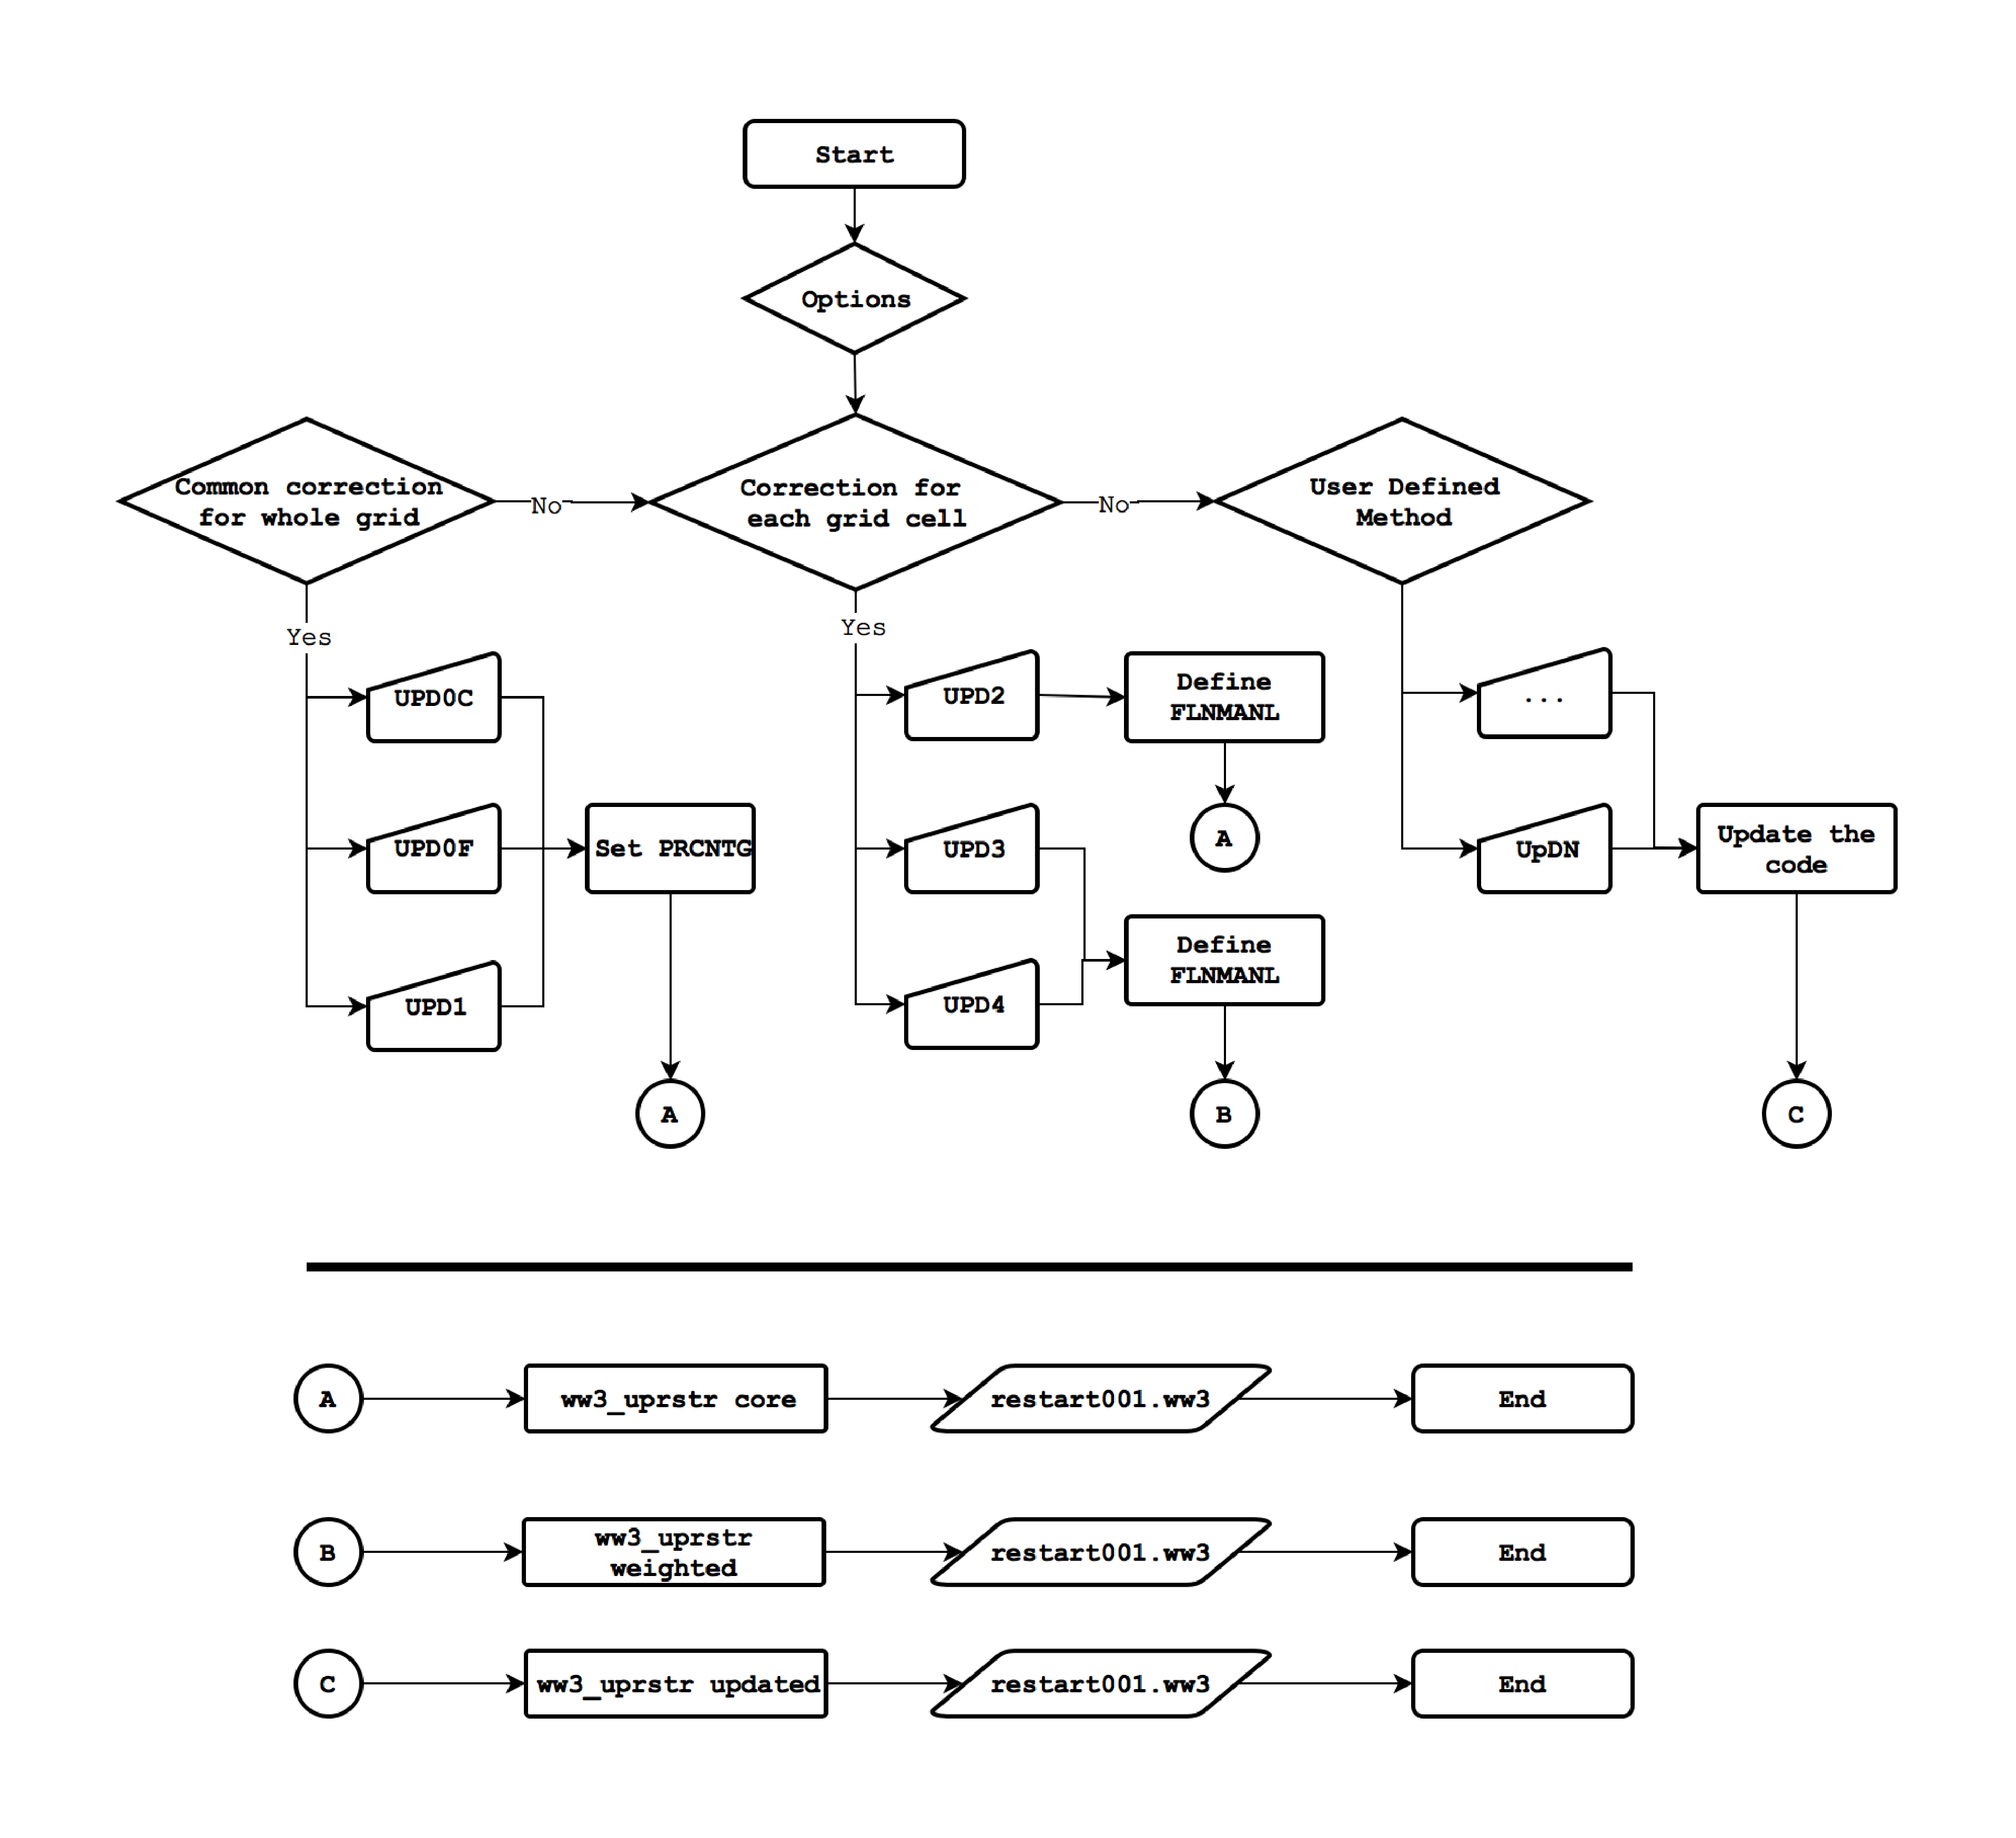
\includegraphics[width=0.9\textwidth]{./run/uprstr.eps}
\caption{Flowchart of the implemented methods for updating the wave spectra at the WW3 
restart file. Additional methods can be implemented by adding UPD options to the namelist.}
\label{fig:uprstrflowchart} \botline
\end{center}
\end{figure}

The following UPD options are available:
\begin{enumerate} 
   \item UPD0C:: \textbf{ELIMINATED from version x.xx} Option 0C  All the spectra are 
   updated with a constant: \newline
      \(fac=(SWH\_Bckg-SWH\_Anl)/SWH\_Anl \).
   \item UPD0F:: Option 0F  All the spectra are updated with a constant: \newline 
      \(fac=SWH\_Anl/SWH\_Bckg \).
   \item UPD1 ::  \textbf{ELIMINATED from version x.xx} Option 1  The fac(x,y,frq,theta), 
   is weighted according to the \% of energy at each spectral bin; fac the same as UPDOF.
   \item UPD2 :: Option 2   The fac(x,y,frq,theta), is calculated at each grid point 
   according to SWH\_Bckg and SWH\_Anl
   \item UPD3 :: Option 3   The update factor is a surface with the shape of 
   the background spectrum. 
   \item UPD4 :: [NOT INCLUDED in the current version, just keeping the spot]
   Option 4  The generalization of the UPD3. The update factor is the sum of surfaces 
   which are applied on the background spectrum. The algorithm requires the mapping 
   of each partition on the individual spectra; the map is used to determine the weighting 
   surfaces.
   \item UPD5 :: Option 5   Corrections are calculated as per UPD2 but are
   applied to wind-sea parts of the spectrum only when wind-sea
   is the dominant component, otherwise the whole spectrum is
   corrected. Required inputs are the the Analysis Hs field plus 
   background wind speed and direction. To include the wind data it is recommended
   to run code built with the WRST switch.
   \item UPD6 :: Option 6   Corrections are calculated as per UPD5 but wind-sea
   components are also shifted in frequency space using Toba (1973).
   Required inputs are the the Analysis Hs field plus background wind speed and direction.
   To include the wind data it is recommended to run code built with the WRST switch.
\end{enumerate}

Any additional method for the redistribution of the energy to the WS and correcting 
the associated winds could be added by further extending the input file and adding 
the source code to the \textbf{ww3\_uprstr.ftn}.

\subparagraph{Example \newline}
In this section, an example of the simplest WDA application is discussed.
The figure ~\ref{fig:waveDAflowchart} shows how the \textbf{ww3\_uprstr} 
is used in the framework of a simple wave analysis system. \newline

A WW3 run (from the previous cycle or from the hindcast) provides the
background field of SWH and the corresponding restart file at the appropriate time. 
The format of the background SWH field has to be compatible with the WDA module inputs.

\begin{figure} \begin{center}
\includegraphics[width=0.9\textwidth]{./run/waveDA.eps}
\caption{Flowchart of simplified wave data assimilation system, 
showing the role of the {ww3\_uprstr}, the required input files,
and the resulted output of the updated restart file.}
\label{fig:waveDAflowchart} \botline
\end{center}
\end{figure}

The WDA module uses the background field and the available observations
for the time of analysis, produces the analysis and exports 
the field of SWH in grbtxt format (\textbf{XXXX.grbtxt}) .

The analysis file, the \textbf{mod\_def.ww3}, the \textbf{restart.ww3} file and 
the \textbf{ww3\_uprstr.inp} are the input files for the \textbf{ww3\_uprstr}. 
If all the options and input files are correctly prepared, it takes approxmately 
one minute to update a grid of 260000 grid nodes and generate the output on a single processor. 
The updated restart file has to be renamed, at the expected file name, in the case of this
example to \textbf{restart.ww3}. \newline  

   \noindent\fbox{
      \parbox{\textwidth}{
      \textbf{Note: }
      All \ncep's WDA systems use GRIB2 format, thereore there is always an intermediate
      step to transfer the grib files to the appropriate format. The used software is WGRIB2 
      and more information can be retrieve from the 
      \href{http://www.cpc.ncep.noaa.gov/products/wesley/wgrib2} {official website}.       
      }
   }

%\paragraph{How to Update the ww3\_uprstr \newline}
%Add data readers, mainly for machine independent binary data and wgrib2.

\pb


% tab:fields

\begin{table} \begin{center}
\begin{tabular}{|c|c|c|c|c|c|} \hline
group & field & description                  &  file        & GRIB1 & GRIB2   \\
      &                              &  extension   & data  & data    \\ \hline \hline
 1 & 1 & depth                           & {\file .dpt} &  --  &    --    \\
 1 & 2 & mean current components         & {\file .cur} &  --  &    --    \\
 1 & 3 & wind speed                      & {\file .wnd} &  32  &  0,2,1   \\
   &&  wind direction                 &              &  31  &  0,2,0   \\
   &&  wind $u$                       &              &  33  &  0,2,2   \\
   &&  wind $v$                       &              &  34  &  0,2,3   \\
 1 & 4 & air-sea temp. dif.              & {\file .dt}  &  --  &    --    \\
 1 & 5 & water level                     & {\file .wlv} &  --  &  10,3,1  \\
 1 & 6 & ice coverage                    & {\file .ice} &  91  &  10,2,0  \\
 2 & 1 & wave height $H_s$               & {\file .hs}  & 100  &  10,0,3  \\
 2 & 2 & mean wave length                & {\file .l}   &  --  &    --    \\
 2 & 3 & mean wave period $T_{m0,2}$     & {\file .t02} &  --  &    --    \\
 2 & 4 & mean wave period $T_{m0,1}$     & {\file .t}   & 103  &  10,0,15 \\
 2 & 5 & mean wave period $T_{m0,-1}$    & {\file .tm1} &  --  &    --    \\
 2 & 6 & peak frequency $f_p$            & {\file .fp}  & 108  &  10,0,11 \\
 2 & 7 & mean wave direction $\theta_m$  & {\file .dir} & 101  &    --    \\
 2 & 8 & directional spread $\sigma$     & {\file .spr} &  --  &    --    \\
 2 & 9 & peak direction $\theta_p$       & {\file .dp}  & 107  &  10,0,10 \\
 4 & 1 & $H_s$ of partition              & {\file .phs} & 102,105 & 10,0,5/8 \\
 4 & 2 & $T_p$ of partition              & {\file .ptp} & 110,106 & 10,0,6/9\\
 4 & 3 & $L_p$ of partition              & {\file .plp} &  --  &    --    \\
 4 & 4 & $\theta_m$ of partition         & {\file .pdir} & 109,104 & 10,0,4/7 \\
 4 & 5 & $\sigma$ of partition           & {\file .psi} &  --  &    --    \\
 4 & 6 & wind sea fraction of part.      & {\file .pws} &  --  &    --    \\
 4 & 7 & total wind sea fraction         & {\file .wsf} &  --  &    --    \\
 4 & 8 & number of partitions            & {\file .pnr} &  --  &    --    \\
 5 & 1 & friction velocity comp.         & {\file .ust} &  --  &    --    \\
 5 & 2 & Charnock par for air side & {\file .cha} &  --  &    --    \\
 5 & 3 & Energy flux $\int C_g E(f) df$  & {\file .CgE} &  --  &    --    \\
 5 & 4 & Wind to wave energy flux        & {\file .faw} &  --  &    --    \\
 5 & 5 & Wave-supported stress           & {\file .taw} &  --  &    --    \\
 5 & 6 & Upward wave-supported stress    & {\file .twa} &  --  &    --    \\
 5 & 7 & Whitecap coeverage              & {\file .wcc} &  --  &    --    \\
 5 & 8 & Avg whitecap foam thickness & {\file .wcf} &  --  &    --    \\
 5 & 9 & Sign breaking wave height& {\file .wch} &  --  &    --    \\
 5 & 10 & Whitecap moment                 & {\file .wcm} &  --  &    --    \\ \hline
\end{tabular} \end{center}
\caption{~Field output post processors ancillary data.} \label{tab:fields}
\vspace{0.5in}
\end{table}

\begin{table} \begin{center}
\begin{tabular}{|c|c|c|c|c|c|} \hline
group & field & description                  &  file        & GRIB1 & GRIB2   \\
      &                              &  extension   & data  & data    \\ \hline \hline
 6 & 1 & radiation stress                & {\file .Sxy} &  --  &    --    \\
 6 & 2 & Breaking wave momentum flux     & {\file .two} &  --  &    --    \\
 6 & 3 & Bernoulli head                  & {\file .J} &  --  &    --    \\
 6 & 4 & Breaking wave energy flux       & {\file .foc} &  --  &    --    \\
 6 & 5 & Stokes transport                & {\file .tus} &  --  &    --    \\
 6 & 6 & Surface Stokes drift            & {\file .uss} &  --  &    --    \\
 6 & 7 & Second order pressure at $k=0$  & {\file .p2s} &  --  &    --    \\
 7 & 1 & near-bottom amplitude           & {\file .cfd} &  --  &    --    \\
 7 & 2 & near-bottom velocity            & {\file .ubr} &  --  &    --    \\
 7 & 3 & bedform parameters              & {\file .bed} &  --  &    --    \\
 7 & 4 & Energy flx to bot bound layer & {\file .fbb} &  --  &    --    \\
 7 & 5 & Momentum flx to bot bound layer & {\file .tbb} &  --  &    --    \\
 8 & 1& mean square slopes              & {\file .mss} &  --  &    --    \\
 8 & 2 & Phillips constant               & {\file .msc} &  --  &    --    \\
 9 & 1 & average time step               & {\file .dtd} &  --  &    --    \\
 9 & 2 & cut-off frequency $f_c$         & {\file .fc}  &  --  &    --    \\
 9 & 3 & cut-off frequency $f_c$         & {\file .fc}  &  --  &    --    \\
 9 & 4 & maximum CFL for X-Y advection   & {\file .cfx} &  --  &    --    \\
 9 & 5 & maximum CFL for $\theta$ advection & {\file .cfd} &  --  &    --    \\
 9 & 6 & maximum CFL for $k$ advection   & {\file .cfk} &  --  &    --    \\
 10 & 1 & user defined \#1                & {\file .us1} &  --  &    --    \\
 10 & 2 & user defined \#2                & {\file .us2} &  --  &    --    \\ \hline
%13 & wind sea period $T_w$           & {\file .fpl} & 110  &    --    \\
%14 & wind sea direction $\theta_w$   & {\file .dpl} & 109  &    --    \\

\end{tabular} \end{center}
\caption*{Table~\ref{tab:fields}, continued.} 
\vspace{0.5in}
\end{table}

\clearpage

%\bpage
